\documentclass[11pt]{article}
\usepackage[utf8]{inputenc}
\usepackage[T1]{fontenc}
\usepackage{amsmath}
\usepackage{amsfonts}
\usepackage{amssymb}
\usepackage[version=4]{mhchem}
\usepackage{stmaryrd}
\usepackage{graphicx}
\usepackage[export]{adjustbox}
\graphicspath{ {./images/} }

\begin{document}
Private Equity Fund Fees and Terms

The session, Quantitative Foundations introduced the fees and terms found in limited partnerships for private structures in general. This lesson provides further detail, especially with respect to features unique to PE.

\section*{Private Equity Management Fees and Carried Interest}
At the heart of the difference between public and PE governance structures are the compensation structures that provide incentives for the managers and investors.

Management fees for PE depend on the size of the fund, generally ranging from $1.5 \%$ of committed capital for large funds to $2.5 \%$ for smaller funds. During the investment period, the management fee is generally assessed on the amount of committed capital, not invested capital. Once the investment period concludes, the management fee should be charged on invested capital, not committed capital. Committed capital is the cash investment that has been promised by an investor.

Consider the implications of this fee arrangement. The manager collects a management fee from the moment an investor signs a subscription agreement to invest capital in the fund, even though no capital has actually been contributed by the LP yet. Further, VC funds typically provide for capital calls. Capital calls are options for the manager to demand, according to the subscription agreement, that investors contribute additional capital. The potential for the manager to earn incentive fees on capital from capital calls may give the manager an incentive to call for capital, even when investment opportunities are not of the highest quality. Capital calls are typically made when each portfolio company investment is identified (and if the VC fund holds insufficient uninvested cash).

General partners can earn a wide variety of fees from their portfolio companies, including director fees, buyout fees, financing fees, divestment fees, and so on, as detailed in the management services agreement between the GP and the portfolio company. There are considerable differences from one fund to the next regarding the level of fees and how those fees are attributed between the GP and the LP. These can have an impact on returns and often account for material differences between gross and net returns. LPs would prefer that all fees earned by the GP would offset the management fees due from the LPs.

The main upside incentive for GPs comes in the form of carried interest, typically $20 \%$ of the profits realized by the fund. Incentive fees are typically entitled carried interest in PE funds and can be calculated on either a fund-as-a-whole or a deal-by-deal basis, as detailed in the session, Quantitative Foundations. In recent years, LPs have been overwhelmingly rejecting deal-by-deal carry. But whether this approach is now really extinct or the pendulum will swing back toward more GPfriendly carried interest mechanisms remains to be seen.

\section*{Private Equity and Clawback Provisions}
Most PE partnership agreements include a clawback provision. A clawback provision, introduced in the session, Quantitative Foundations, is a covenant that allows the LPs to receive back (or claw back) previously paid incentive fees. The previously paid incentive fees are returned if, at the end or liquidation of the venture fund, the LPs have returns below the annualized preferred return. There is often a clawback escrow agreement, in which a portion of the manager's incentive fees are held in a segregated account until the entire fund is liquidated. This ensures that the fund manager does not walk away with incentive fees unless the LPs earn a profit in excess of the hurdle rate or the preferred return. Only after every limited partner has earned a profit are the escrow proceeds released to the manager. Sometimes this covenant may stipulate that all management fees must also be recouped by the LPs before the manager can collect incentive fees.

Responsibility for payment of the clawback rests with the persons or entity that received the carried-interest distributions. In such a case, the GP is required to return some proceeds to make the investor whole. But clawback can also exist for LPs. In this case, it is triggered when, at the end of a fund's life, the GPs have received less than their share of the fund's profits. Such clawback is relevant in situations in which a portion of the committed capital has not been drawn, and LPs have received full repayment of their commitment plus hurdle before the GP has access to his or her carry.

The simplest and, from the viewpoint of an LP, most desirable solution is that GPs do not take carried interest until all invested, or sometimes even all committed, capital has been repaid to investors. In this scenario, however, the several years it could take for the fund's team to see any gains could lead to demotivation. Accordingly, carried interest is usually distributed to GPs as profits are realized. A clawback ensures that managers will not receive a greater share of the fund's distributions than they are entitled to.

\section*{Private Equity Carried Interest and Hurdle Rates}
In the case of PE, carried interest can be subject to a hurdle rate, or preferred return, so that it begins to accrue only once investors have received their capital back and a minimum previously agreed-on rate of return. Once the preferred return has been attained, GPs typically receive $100 \%$ of returns to the point at which they have received the carried interest on the entire amount. This is called a catch-up and is synonymous with the soft hurdle concept used by hedge funds and detailed in the session, Quantitative Foundations. The exhibit below illustrates the effect of hurdle rates with a catch-up clause.

\begin{center}
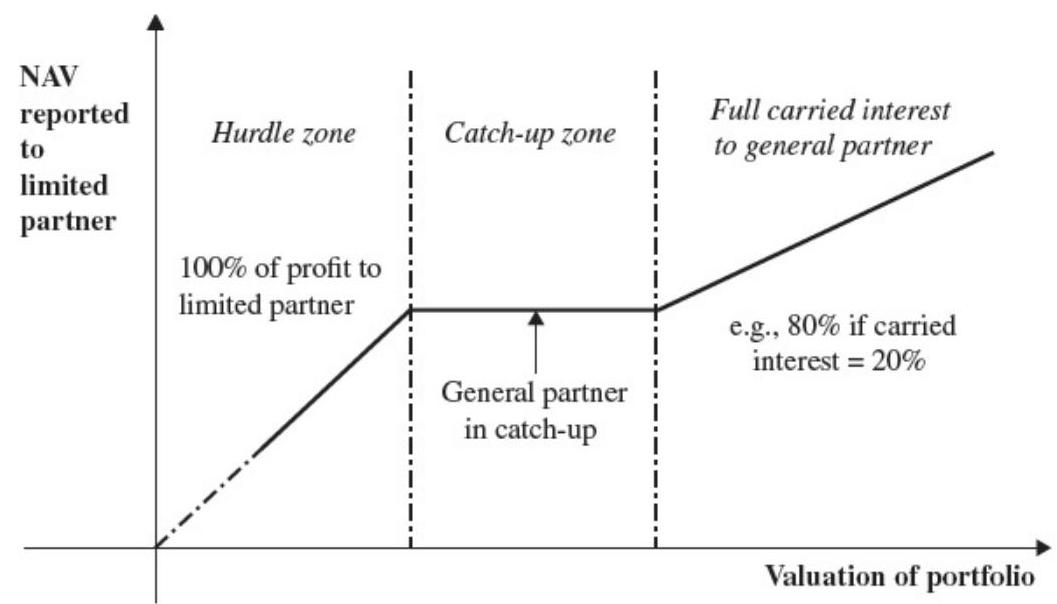
\includegraphics[max width=\textwidth]{2024_04_10_afcfe94612d988da8947g-3}
\end{center}

Impact of Catch-Up on NAV Attributed to LPs

In the exhibit above the function that maps the value of the portfolio to the net asset value (NAV) contains three segments from left to right. In the hurdle zone, the LPs receive all the cash inflows. This is followed by the catch-up period, during which the GP receives all or the major share of distributions. As discussed in the next section, these zones can cause unintended consequences. The catch-up period ends when the agreed-on carried-interest split, or stated share of the fund's profits to be received by the GP and the LPs, is reached. Thereafter, distributions are shared between the fund manager and investors in the proportion agreed to in the legal documentation, normally $20 \%$ for the GP and $80 \%$ for LPs.

These mechanisms for carried interest payments are not standardized (e.g., whether an interest rate such as a hurdle rate is compounded on a quarterly or on an annual basis). Sometimes there is a full catch-up, whereas other agreements may foresee only a partial catch-up or no catch-up at all. With a $100 \%$ catch-up, the LPs are effectively excluded from all new distributions until the GP has fully recovered the agreed-on GP share of the profit.

The exhibit below provides a numerical example that brings together many of the components of the cash waterfall that were introduced in the session, Quantitative Foundations. To simplify, assume a $€ 100$ million contribution by the LPs in the first year to fund an investment, an $8 \%$ hurdle rate, a 100\% catch-up, an $80 / 20$ carry split, and the sale of the investment by the fund in the second year for $€ 200$ million. In this case, the sales proceeds are distributed as shown in Example of Waterfall Using a Hurdle Rate exhibit below. The $€ 2$ million catchup for the GP is found by ensuring that the GP gets $20 \%$ of the total, which is $25 \%$ of the LPs' payout. The $25 \%$ figure is found as: $20 \% /(1-20 \%)$ where $20 \%$ is the GP's share.

Note that simply splitting the profit of $€ 100$ million (the difference of $€ 200$ million in sales proceeds minus the $€ 100$ million purchase price) on an $80 / 20$ basis would have given the same result. The reason for this is that the fund's return is above the catch-up zone, and therefore the hurdle is extinguished and does not make any difference.

\begin{center}
\begin{tabular}{|c|c|c|c|}
\hline
\multicolumn{4}{|c|}{Example of Waterfall Using a Hurdle Rate} \\
\hline
 & LPs & GP & Total \\
\hline
Original contribution & $-€ 100$ million &  & $-€ 100$ million \\
\hline
\multicolumn{4}{|l|}{Sale of investment for $€ 200$ million} \\
\hline
Return of capital & $€ 100$ million &  & €100 million \\
\hline
Preferred return for limited partners & €8 million &  & €8 million \\
\hline
Catch-up for GP &  & $€ 2$ million & $€ 2$ million \\
\hline
80/20 split of residual amount & $€ 72$ million & $€ 18$ million & $€ 90$ million \\
\hline
Closing balance & $€ 80$ million & $€ 20$ million & $€ 100$ million \\
\hline
\end{tabular}
\end{center}

\section*{Private Equity Perverse Incentives from Fees}
There are two potentially major perverse incentives generated by hurdle rates.

First, high hurdle rates can cause excessive risk taking. Managers of funds with overly high hurdle rates (or of struggling funds) can become unmotivated if it becomes unlikely that they will receive carried interest. When the GP's call-option-like incentive fee moves far out-of-the-money, the high hurdle rates may lead to desperate\\
risk taking. The option-like payoffs to GPs may mean that the more risk a manager takes, the greater the upside potential, with little immediate downside impact from losses. This is why the GP's capital contribution (discussed in the next section) is so important.

There are also some timing issues with hurdle rates (preferred returns). GPs are faced with the dilemma of whether to realize an investment over a short period of time to optimize the spread of the IRR over the hurdle rate or to hold on to the investment and try to optimize the long-term multiple. For example, is it better to generate a 50\% IRR for a period of three months, which yields a $1.11 \times$ multiple on capital invested, or only a $10 \%$ IRR for a period of three years, leading to a $1.33 \times$ multiple? The standard preferred return, being based on the IRR, gives incentive to the former. To the extent that GPs game the timing of the investment realizations based on the effect of the timing decision on the carried interest split, it is likely that the LPs suffer adverse consequences.

Investors need to read the limited partnership agreement carefully, as there is a potential for substantial conflicts of interest between the GP and the LP. If LPs don't understand the terms, the GPs may earn much larger fees than those that are clearly stated (such as 2 and 20 over 8\%). There has been an increasing use of subscription lines, which are lines of credit used by the GP to make investments in portfolio companies. If subscription lines are used to delay capital calls and reduce the time that LPs are invested in the fund, the IRR of the fund may be higher than if capital calls were made at the time the investments were made in the portfolio company.

\section*{GP's Contribution to Initial Private Equity Fund Investment}
Excessive risk taking can be reduced or eliminated if managers have a significant portion of their personal wealth in the fund. In this case the manager, being directly exposed to fund losses, has little or no incentive to take excessive risks, to work on non-fund-related activities, or to abandon ship once the prospects for generating carry and launching a follow-on fund become highly unlikely.

Typically, investors in PE funds see $1 \%$ of the fund's committed capital as a standard and acceptable contribution for GPs to make. The capital contribution by GPs, also known as hurt money, should be contributed in cash rather than through the waiver of management fees (or as surplus from the management company's budget). However, in the case of wealthy managers, $1 \%$ may at times be too low, as LPs prefer that the GP contribution be at a level that is a substantial portion, perhaps one-quarter to one-half, of the personal net worth of the top partners of the fund management company.

To better understand this relationship, it makes sense to look at the GP's and LPs' relative exposure. Typically, the GP's contribution to the fund is a significant share of his or her personal wealth, whereas the LPs' investment, although in absolute terms is far higher, represents an immaterial share of the institution's overall assets. It is a challenge to determine the appropriate contribution level for a GP: one that provides a reasonable incentive but is not excessively onerous. An analysis of profits earned from past investments, salaries, budget surpluses, and so forth may provide useful information for determining a contribution level that is appropriate for a particular GP.

\section*{Key-Person Provision}
PE is to a large degree a people business. Depending on the size, experience, and depth of the team, the inability of one or several key persons to carry out their duties could have a substantial adverse effect on the partnership. Consequently, the key-personnel clause is a common and important clause in partnerships that allows LPs to take specified actions in the event that one or several of the named key persons depart the team, stop committing sufficient time to the management of the fund, or sell their interests in the management company.

The key-personnel (or key-person) clause (or provision) allows LPs to suspend investment and/or divestment activities until a replacement or replacements are found. The LPs may even be able to terminate the fund if they so choose. Key-person clauses may also be put in place in anticipation of the retirement of senior fund managers.

\section*{Termination and Divorce}
LPs may include a bad-leaver clause, which is a for-cause removal of the GP that, if exercised (normally following a simple majority vote of the LPs), causes investments to be suspended until a new fund manager is elected or, in the extreme, the fund is liquidated. In practical terms, conditions leading to a for-cause removal are difficult to both define and determine. In PE, ultimately very little is legally enforced; issues are highly subjective, and taking matters to court carries high legal risk for an investor, as it is very difficult and lengthy to prove wrongdoing.

A good-leaver clause enables investors to cease additional funding of the partnership with a vote requiring a qualified majority (generally more than $75 \%$ of LPs). This "without-cause" clause provides a clear framework for shutting down a partnership that is not working, or when confidence is lost. The good-leaver clause sometimes provides for compensation amounting to six months to one year of management fees; the bad-leaver clause provides no such compensation and foresees no entitlement to carried interest.

In deciding whether to exercise one of these clauses, reputation considerations play a key role, as the market consists of a small number of players who repeatedly interact with one another. GPs who are removed with or without cause may subsequently be unable to raise funds or participate in investment syndicates with other partnerships. To avoid such disastrous outcomes, GPs tend to agree on a fund restructuring to prevent a forced removal.

\section*{Other Covenants}
The terms of the partnership agreements of VC funds contain details regarding the partnership's funding, the distribution of cash, the operation of the fund, the investment practices of the fund, and various covenants.

Typically, the most important covenant is the size of an investment by the VC fund in any one start-up venture, usually expressed as a percentage of the capital committed to the VC fund. The purpose is to ensure that the manager does not commit too much capital to a single investment. In any VC fund there will be start-up ventures that fail to generate a return. By diversifying across several venture investments, this risk is mitigated.

Other covenants may include a restriction on the use of debt or leverage by the fund. VC investments are risky enough without the manager gearing up the fund through borrowing. Gearing is a term for increasing risk through leverage. In addition, there may be a restriction on co-investments (detailed in Level 2 of the CAIA curriculum) with prior or future funds controlled by the manager. Furthermore, there is usually a covenant regarding the distribution of profits. Investors find that it is\\
optimal for them to receive the profits as they are realized. Distributed profits reduce the amount of committed capital in the venture fund, which in turn reduces the fees paid to the manager. It is in the VC fund manager's economic interest to retain profits.

Primary among restrictions on the general partner's activities is a limit on the amount of private investments the VC fund manager can make on its own in any of the firms funded by the VC fund. If the VC fund manager makes private investments in a select group of companies, these companies may receive more attention than the remaining portfolio of companies funded by the VC fund. GPs are often limited in their ability to sell their general partnership interests in the VC fund to a third party. Such a sale would be likely to reduce the general partner's incentive to monitor investments and produce an effective exit strategy for the VC fund's portfolio companies.

Two other covenants also relate to keeping the manager's focus on managing the fund. The first is a restriction on the amount of future fundraising. Fundraising is time-consuming and can detract from the manager's time spent managing the investments of the existing fund. Also, LPs typically demand that the general partner spend substantially all of the time managing the investments of the fund; outside interests are limited or restricted.

There are often additional covenants that keep VC fund managers focused on investing in those companies, industries, and transactions in which they have the greatest experience. For instance, there may be restrictions or prohibitions on investing in buyouts, other VC funds, foreign securities, or companies and industries outside the realm of the manager's expertise.


\end{document}